\iffalse \bibliography{include/backmatter/magnus,include/backmatter/philip} \fi
\chapter{Use-Case Scenario}\label{section:data-validation}

This section introduces the result of executing parts of the experiment on a self-driving Volvo truck, depicted in figure~\ref{truck}, that participated in the Grand Cooperative Driving Challenge (GCDC) 2016 in the Netherlands. As the use-case scenario is an uncontrolled environment, the experiment conducted on the self-driving Volvo truck is not intended to answer the research questions of this research, rather to provide an understanding of how the scheduling precision of the experimental unit; Pi Component (section~\ref{section:exp-units-pi}) is impacted by the deployment context in a system with an operational full-scale vehicular CPS running simultaneously.\\

\begin{figure}[ht]
\centering
\caption{Chalmers Revere GCDC Truck}
\label{truck}
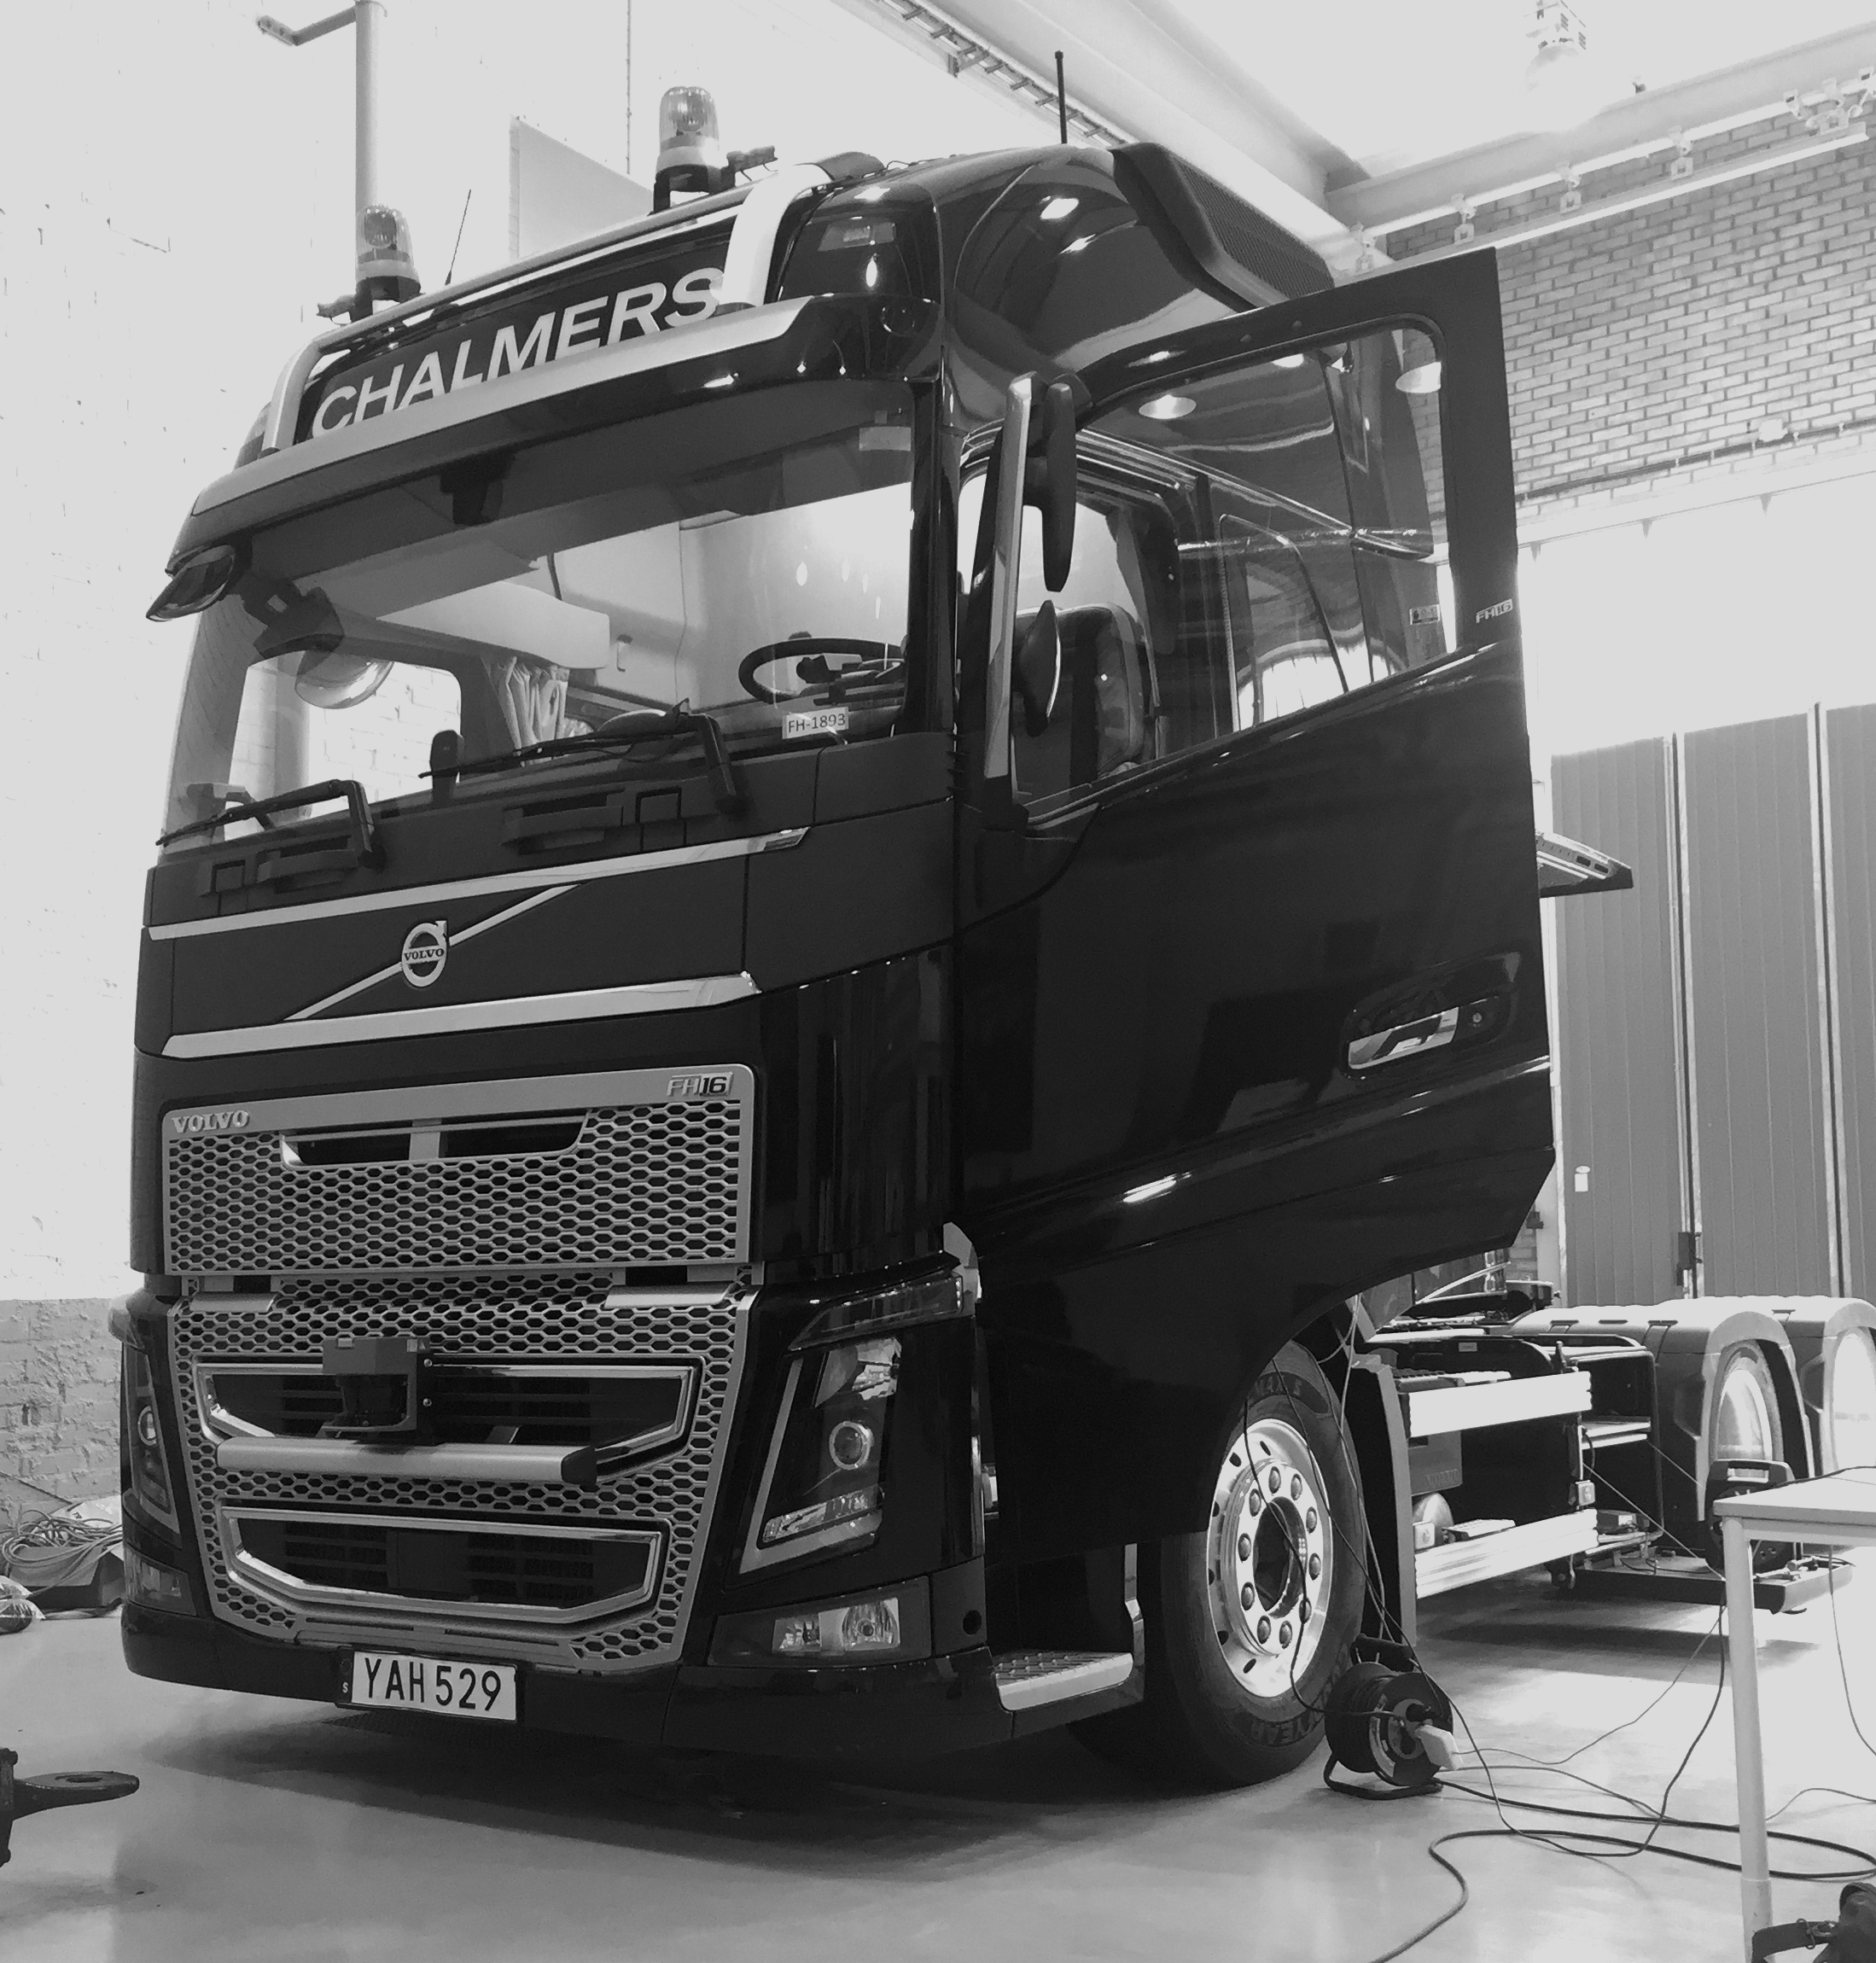
\includegraphics[width=0.4\textwidth]{./figure/truck.png}
\end{figure}


\section{Method}
\label{sec:truck-method}

This section is aimed at providing the method of the experiment conducted on the uncontrolled environment of the use-case scenario.


\subsection{Experimental Units}
\label{sec:truck-expun}

The Pi Component from \ref{section:exp-units} is executed on a target system identical to the one used during the controlled experiments. The computer is connected to hardware components mounted to a Volvo FH16 truck. As the use-case data is extracted using the Pi Component no measurements are done to understand the camera input and disk output performance for the use-case due to the priority of building an understanding of how the scheduling precision behaves with the runtime load of the self-driving truck.\\

To understand how Docker impacts the scheduling precision on the use-case, the experimental unit is executed first natively and secondly within a Dockerised container. The runtime properties of Docker are presented in table \ref{docker-parameters-truck}. Docker version 1.11.1 is used for the analysis procedure and the Docker daemon is set to use the \texttt{overlayfs} storage driver.



\begin{table}[ht]
\centering
\caption{Docker Image Runtime Properties}
\label{docker-parameters-truck}
\begin{tabular}{|l|p{10cm}|}
\hline
\textbf{Parameter}           & \textbf{Description}                                            \\ \hline
\texttt{-d}                  & Run the container in detached mode.                             \\ \hline
\texttt{--net=host}          & The networking configuration is derived from the host.          \\ \hline
\texttt{--cap-add=sys\_nice} & Allow access to devices such as the web camera and the serial port. \\ \hline
\texttt{-v}                  & Mount shared filesystems from the host into the container.    \\ \hline
\texttt{-w}                  & The working directory to execute the experimental units.               \\ \hline
\end{tabular}
\end{table}


\subsection{System Load}
\label{sec:truck-load}

The major difference in comparison to the controlled experiment run is that all software components required for the Volvo truck to operate in a driver-less manner is started and run in the background: this bring a more realistic operational load and consequently a less controlled environment in respect to the controlled experiment. Fifteen components are executed natively and within a Dockerized environment on the target system. These components are tasked with various responsibilities spanning from capturing satellite positioning data, reading data from the vehicle (e.g steering position), vehicle to vehicle communication and a number of camera operating components. Measurement points are captured via serial communication to measure the impact in a real use case.\\

\subsection{Target System}
\label{sec:truck-target}

Table \ref{table:hardware-truck} presents the hardware setup for the target machine upon which the experimental unit (section \ref{sec:truck-expun}) is executed. The target system is running ArchLinux operating system with a real-time enabled kernel (RT\_preempt), version 4.5.0-1.

\begin{table}[H]
\centering
\caption{Target System Hardware Specification}
\label{table:hardware-truck}
\begin{tabular}{|l|l|}
\hline
\textbf{Component} & \textbf{Specification}           \\ \hline
Processor          & Intel Core i7 3517UE 1.7 GHz     \\ \hline
Memory             & 4GB DDR3 1333/1600 SODIMM        \\ \hline
Storage Device     & 2.5" SATA HDD x 1                \\ \hline
Serial Interfaces  & \begin{tabular}[c]{@{}l@{}}USB type A x 2 for USB 2.0\\ USB type A x 2 for USB 3.0\\ DB-9 x 2 for RS-232/422/485 x 2\\ DB-9 x 4 for RS-232 x 4 \\ Isolated DB-9 x 2 for RS-232/422/485 x 2
\end{tabular} \\ \hline
\end{tabular}
\end{table}


\subsection{Variables}

The uncontrolled experiment is intended to understand the deployment context's impact on the scheduling precision. In comparison to the controlled environment the kernel version is not controlled and thus not used as a treatment to the use-case experiment. The deployment context is a categorical variable which holds two values, namely 1) Native and 2) Docker. Where the former is executing the experimental unit on the host OS and the second is executing it in a Dockerized container. As the use-case scenario is a replication of the controlled environment, the same dependent variables are used for measuring the scheduling precision of the experimental unit, namely: 1) Overhead \#1, 2) Pi Algorithm, 3) Overhead \#2, and 4) Sleep. Figure \ref{pi_measure} presents the measurement points from where within the time-slice each of the dependent variables are extracted.\\


\subsection{Procedure}

The procedure is to execute the experimental unit in 2 different scenarios. The two scenarios is an alternation between two deployment contexts, namely 1) Executing natively on the host OS, and 2) Executing within a Dockerized environment. Each scenario is manually executed for $1h$ on the target machine with the Raspberry Pi SoC \cite{raspberry} hardware connected through a serial to USB device used for capturing measurement data via RS-232 serial communication.\\


\subsection{Analysis Procedure}

Analysing the data is made with a partly replicated analysis procedure used for understanding the scheduling precision of the controlled experiment. In contrast to the controlled experiment the results of the use-case scenario does not seek to answer any hypotheses or research questions, therefore the MANOVA has been excluded. The purpose is rather to provide an insight to how the experimental unit's scheduling precision behaves in a environment with realistic load. Each of the measurement points presented in figure \ref{pi_measure} are extracted and processed by calculating the duration between the points using a script. The durations is then analysed by building bar charts to illustrate the scheduling precision which is intended to provide an overview of all data points extracted. Furthermore, a table of sample size, means, and standard deviations is constructed to provide the descriptive statistics of the generated bar charts. Lastly, the effect size ($\eta^{2}$) between the deployment context and scheduling precision is calculated to bring a more detailed understanding of what impact the deployment context has on the scheduling precision.\\








